% !TeX spellcheck = it_IT
\newpage
\section{Normalizzazione}
Dati diversi modelli relazionali e diverse possibili rappresentazioni sorge il problema di verificare se:
\begin{itemize}
	\item queste diverse rappresentazioni sono tra di loro \textbf{equivalenti}
	\item queste rappresentazioni sono di \textbf{buona qualità} (assenza di \textbf{anomalie})
\end{itemize}

\begin{definition}[Teoria della normalizzazione]
	La teoria della normalizzazione si occupa di \textbf{definire criteri formali} per giudicare l’\textbf{equivalenza} di schemi e la \textbf{qualità} di tali schemi, e di definire algoritmi per trasformare uno schema in un altro equivalente ma privo di anomalie.
\end{definition}

\subsection{Linee guida}
Ci sono quattro principali linee guida per avere una corretta progettazione:
\begin{itemize}
	\item \textbf{Semantica degli attributi}: si devono progettare schemi relazionali in modo tale che sia semplice spiegarne il significato evitando di unire attributi provenienti da più tipi di classi e tipi di associazione in una unica relazione.
	\item \textbf{Ridondanza}: si devono progettare schemi relazionali in modo che nelle relazioni non
	siano presenti anomalie di inserimento, cancellazione o modifica. Se sono presenti (e le si vuole mantenere), le si rilevi e ci si assicuri che i programmi che aggiornano la BD operino correttamente
	\item \textbf{Valori nulli}: evitare di porre in relazione di base attributi i cui valori possono essere spesso nulli. Se è inevitabile, assicurarsi che essi si presentino solo in casi eccezionali e che non riguardino una maggioranza di tuple nella relazione.
	\item \textbf{Tuple spurie}: si devono progettare schemi relazionali in modo tale che essi possano
	essere riuniti tramite giunzioni con condizioni di uguaglianza su attributi	che sono o chiavi primarie o chiavi esterne in modo da garantire che	non vengano generate tuple spurie. Evitare relazioni che contengono attributi di giunzione diversi dalle combinazioni chiave esterna-chiave primaria.
\end{itemize}

\subsubsection{Anomalie}
Le principali anomalie che si trovano sono:
\begin{itemize}
	\item \textbf{Ridondanze}
	\item Potenziali \textbf{inconsistenze}
	\item Anomalie nelle \textbf{inserzioni}
	\item Anomalie nelle \textbf{eliminazioni}
\end{itemize}

\begin{example}
	Supponiamo di avere una BD di una biblioteca
	\begin{center}
		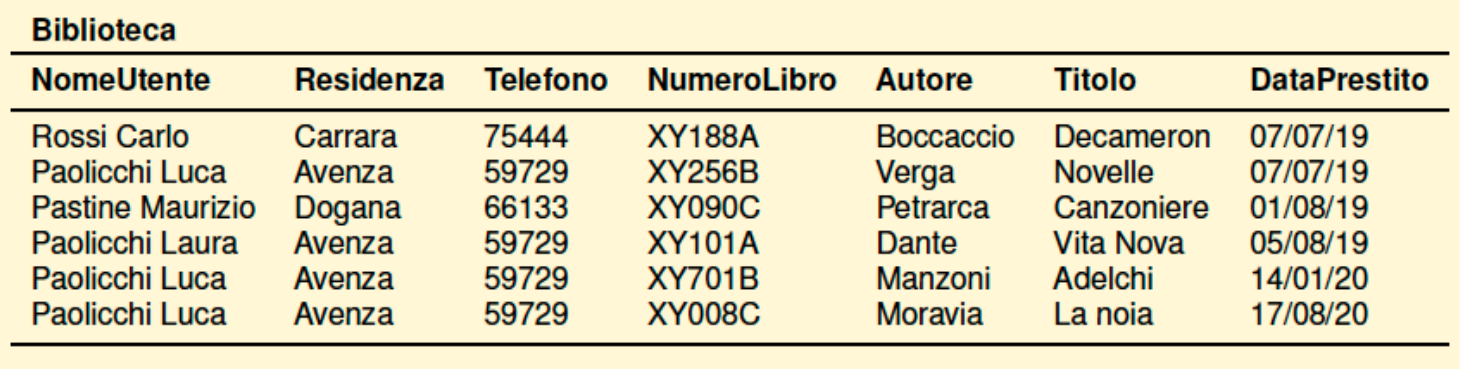
\includegraphics[scale=0.3]{biblioteca1.png}
	\end{center}
	Questo schema presenta due anomalie:
	\begin{itemize}
		\item \textbf{Ridondanza} delle informazioni personali di un utente
		\item Impossibilità di rappresentare le informazioni sugli utenti della biblioteca che non hanno preso in prestito libri
	\end{itemize}
	Una possibile soluzione è la \textbf{decomposizione} in due relazioni:
	\begin{lstlisting}[language=SQL]
		Utenti(NomeUtente, Residenza, Telefono)
		Prestiti(NumeroLibro, Autore, Titolo, Data, NomeUtente*)
	\end{lstlisting}
	Non è la soluzione migliore per costo di operazioni ma funziona.
\end{example}

\subsubsection{Obiettivi}
L'obiettivo della normalizzazione è fornire \textbf{strumenti formali} per la progettazione di basi di dati che non presentino anomalie senza prendere in considerazione il costo delle operazioni. In particolare si occupa di:
\begin{itemize}
	\item \textbf{Equivalenza di schemi}: definire quando due schemi sono equivalenti
	\item \textbf{Qualità degli schemi}: definire quando uno schema è migliore di un altro
	\item \textbf{Trasformazione degli schemi}: trovare metodi algoritmici per ottenere da uno schema uno migliore ed equivalente
\end{itemize}

\subsubsection{Schema di relazione universale}
\begin{definition}[Schema di relazione universale]
	Assumendo come \textbf{ipotesi} che tutti i fatti sono descritti da attributi di un’unica relazione
	(relazione universale), cioè gli attributi hanno un significato globale.\\
	\textbf{Definiamo} lo schema di relazione universale U come di una base di dati relazionale ha come attributi l’unione degli attributi di tutte le relazioni della base di dati.
\end{definition}

\subsubsection{Notazione}
Di seguito la notazione di base:
\begin{itemize}
	\item \textbf{Singoli attributi}: $A,B,C, A_1, A_2, \ldots$
	\item \textbf{Insiemi di attributi}: $T,X,Y,X_1, \ldots$
	\item \textbf{Abbreviazioni}:
	\begin{itemize}
		\item $XY \equiv X \cup Y$
		\item $AB \equiv \{A, B\}$
		\item $A_1, A_2, \ldots, A_n \equiv \{A_1, A_2, \ldots, A_n\}$
		\item $XA \equiv A \cup \{A\}$
	\end{itemize} 
	\item \textbf{Schema di relazione}: $R(T)$, $r$ la sua \textbf{istanza} e $t$ l'\textbf{ennupla} dell'istanza
	\item Se $X \subseteq T$ allora $t[X]$ indica l'\textbf{ennupla} ottenuta da $T$ considerando solo gli attributi in $X$
\end{itemize}


\subsection{Dipendenze funzionali}
Informalmente, una dipendenza funzionale indica che dato un insieme di attributi, questi ne determinano in maniera univoca altri.

\begin{definition}[Dipendenza funzionale]
	Dato uno schema $R(T)$ e $X, Y \subseteq T$, una dipendenza funzionale è un vincolo su $R$ del tipo $X \to Y$ se:
	\begin{itemize}
		\item $\forall r$ istanza valida di $R$
		\item $\forall t_1, t_2 \in r . t_1[X] = t_2[X] \Rightarrow t_1[Y]=t_2[Y]$
	\end{itemize}
\end{definition}
\newpage
\begin{example}
	Data la seguente tabella
	\begin{table}[!h]
		\centering
		\begin{tabular}{|c|c|}
			\hline
			\textbf{Matricola} & \textbf{Cognome}\\
			\hline
			1 & Rossi \\
			\hline
			2 & Verdi \\
			\hline
			3 & Rossi \\
			\hline
			4 & Viola \\
			\hline
		\end{tabular}
	\end{table}
	esiste la dipendenza funzionale $\text{Matricola} \to \text{Cognome}$
\end{example}

\begin{note}
	Essendo definite solo all'interno di una relazione non possono esistere fra attributi di relazioni diverse.
\end{note}
\begin{note}
	Sono proprietà \textbf{intensionali}, quindi legate al significato dei fatti. Non è possibile dedurle dall'osservazione di alcune istanze.
\end{note}

\begin{definition}[Dipendenza funzionale atomica]
	Ogni DF del tipo $X \to A_1, A_2, \ldots, A_n$ si può scomporre in $X\to A_1, X \to A_2, \ldots, X\to A_n$. DF del tipo $X \to A$ sono dette \textbf{atomiche}.
\end{definition}

\begin{example}
	Dato lo schema
	\begin{equation*}
		\text{DotazioniLibri}(\text{CodiceLibro}, \text{NomeNegozio}, \text{IndNegozio}, \text{Titolo}, \text{Quantità})
	\end{equation*}
	la dipendenza funzionale
	\begin{equation*}
		\text{CodiceLibro}, \text{NomeNegozio}\to \text{IndNegozio}, \text{Titolo}, \text{Quantità}
	\end{equation*}
	si può scomporre in
	\begin{align*}
		& \text{CodiceLibro}, \text{NomeNegozio}\to \text{IndNegozio} \\
		& \text{CodiceLibro}, \text{NomeNegozio}\to \text{Titolo}\\
		& \text{CodiceLibro}, \text{NomeNegozio}\to \text{Quantità}
	\end{align*}
\end{example}

\begin{definition}[Dipendenza funzionale banale]
	Una DF $X \to A$ è detta \textbf{banale} se $A \in X$.
\end{definition} 

\subsubsection{Chiavi}
Le dipendenze funzionali sono una generalizzazione del vincolo di chiave e superchiave. Infatti, dato uno schema $R(T)$, $X,Y \subseteq T$ e $r$ istanza di $R$, se $r \models X \to Y$ allora se $X$
\begin{itemize}
	\item \textbf{Non} è \textbf{superchiave} allora ho un'\textbf{anomalia}
	\item È \textbf{superchiave}, allora $\forall r . r\models X \to T$
	\item È \textbf{chiave}, allora $\forall r. r\models X \to T$ e $X \to T$ è una DF \textbf{completa}
\end{itemize}

\subsubsection{Utilizzo}
Le dipendenze funzionali vengono utilizzate per specificare il significato dei fatti rappresentati in uno schema trovando eventuali anomalie e normalizzandolo. Per questo motivo da ora saranno incluse nella definizione:
\begin{equation}
	R(T,F)
\end{equation}

\paragraph{Dipendenze derivate}
Dato uno schema $R(T,F)$, le sue istanza soddisfano le DF e anche quelle derivabili da esse. Ad esempio dato
\[
R(T,F=\{X \to Y, X \to Z\}) \qquad X,Y,Z \subseteq T, W \subseteq X
\]
allora anche $X \to W$ e $X \to YZ$ saranno soddisfatte:
\begin{itemize}
	\item la prima è ovvia in quanto $W$ è sottoinsieme di $X$
	\item se $t_1[X] = t_2[X]$  allora $t_1[Y] = t_2[Y] \land t_1[Z] = t_2[Z]$ e quindi $t_1[YZ] = t_2[YZ]$
\end{itemize}
\begin{definition}[Implicazione di dipendenze]
	Dato $R(T)$ e dato $F$, diciamo che $F \models X \to Y$ ($F$ implica logicamente $X \to	Y$), se ogni istanza $r$ di $R(T)$ che soddisfa $F$ soddisfa anche $X \to Y$.
\end{definition}

\paragraph{Assiomatizzazione}
Sia $RI$ un insieme di regole di inferenze per $F$, ovvero per derivare altre DF a partire da $F$. Indichiamo con $F \vdash X \to Y$ il fatto che $X \to Y$ sia derivabile da $F$ usando $RI$. L'insieme $RI$ è:
\begin{itemize}
	\item \textbf{Corretto}: se $X \to Y$ è derivabile da $F$ allora ogni istanza che soddisfa $F$ soddisfa anche $X \to Y$
	\begin{equation*}
		F \vdash X \to Y \Longrightarrow F \models X \to Y
	\end{equation*}
	\item \textbf{Completo}: se ogni istanza che soddisfa $F$ soddisfa anche $X \to Y$ implica che $X \to Y$ è derivabile da $F$
	\begin{equation*}
		F \models X \to Y \Longrightarrow F \vdash X \to Y
	\end{equation*}
\end{itemize}

\paragraph{Regole di inferenza}
Gli assiomi di Armstrong (1974) sono il più noto insieme \textbf{corretto} e \textbf{completo} di regole di inferenza per DF:
\begin{itemize}
	\item \textbf{Riflessività}
	\begin{equation}
		Y \subseteq X \Longrightarrow X \to Y
	\end{equation}
	\item \textbf{Arricchimento}
	\begin{equation}
		X \to Y, Z \subseteq T \Longrightarrow XZ \to YZ
	\end{equation}
	\item \textbf{Transitività}
	\begin{equation}
		X \to Y, Y \to Z \Longrightarrow X \to Z
	\end{equation}
\end{itemize} 

\begin{definition}[Derivazione]
	Una \textbf{derivazione} di $f$ da $F$ è una sequenza finita $f_1, \ldots, f_m$ di dipendenze dove $f_m = f$ e ogni $f_i$ è un elemento di $F$ oppure è ottenuta dalle	precedenti dipendenze delle derivazione $f_1, \ldots, f_{i-1}$ usando regole di inferenza.\\
	Una \textbf{sottosequenza} $f_1, \ldots, f_k$ per una derivazione $f_1,\ldots, f_m$ è anch’essa	una derivazione, quindi $F \vdash f_k \forall k = 1, \ldots, m$.
\end{definition}
Sia $F$ un insieme di DF, diremo che $X \to Y$ sia \textbf{derivabile} da $F$ ($F \vdash X \to Y$), se $X \to Y$ può essere inferito da $F$ usando gli assiomi di Armstrong.\\
Vediamo altre regole di derivazione ottenute dagli assiomi di Armstrong:
\begin{itemize}
	\item \textbf{Unione}: $\{X \to Y, X \to Z\} \vdash X \to YZ$
	\begin{enumerate}
		\item  $X \to Y$ per ipotesi
		\item $X \to XY$ per arricchimento da 1
		\item $X \to Z$ per ipotesi
		\item $XY \to YZ$ per arricchimento da 3
		\item $X \to YZ$ per transitività da 2, 4
	\end{enumerate}
	\item \textbf{Decomposizione}: $\{X \to YZ\} \vdash X \to Y$
	\begin{enumerate}
		\item $X \to YZ$ per ipotesi
		\item $YZ \to Y$ per riflessività da $Y \subseteq YZ$
		\item $ X \to Y$ per transitività da 1, 2
	\end{enumerate}
	\item \textbf{Indebolimento}: $\{X \to Y\} \vdash XZ \to Y$
	\begin{enumerate}
		\item $X \to Y$ per ipotesi
		\item $XZ \to X$ per riflessività da $X \subseteq XZ$
		\item $ XZ\to Y$ per transitività da 2, 1
	\end{enumerate}
	\item \textbf{Identità}: $\{\} \vdash X \to X$
\end{itemize}
\newpage
\begin{theorem}
	Gli assiomi di Armstrong sono \textbf{corretti} e \textbf{completi}.
\end{theorem}
\begin{proof}
	Se una dipendenza è derivabile con gli assiomi di Armstrong allora è anche implicata logicamente (correttezza degli assiomi), e viceversa se una dipendenza è implicata logicamente allora è anche derivabile dagli assiomi (completezza degli assiomi).
	\begin{itemize}
		\item Correttezza
		\begin{equation}
			\forall f \qquad F \vdash f \Longrightarrow F \models f
		\end{equation}
		\item Completezza
		\begin{equation}
			\forall f \qquad F \models f \Longrightarrow F \vdash f
		\end{equation}
	\end{itemize}
\end{proof}

 \subsubsection{Chiusura}
 La \textbf{chiusura} è l’insieme di DF $X \to Y$ derivabili da $F$.
\begin{definition}[Chiusura]
	Dato un insieme $F$ di DF, la sua chiusura, denotata con $F^+$ è
	\begin{equation}
		F^+ = \{ X \to Y \vert F \vdash X \to Y\}
	\end{equation}
\end{definition}

La chiusura di $X$ rispetto ad $F$ è l’insieme di attributi determinati da $X$ tra quelli delle DF derivabili da $F$.
\begin{definition}[Chiusura]
	Dato $R(T, F)$, e $X \subseteq T$, la chiusura di $X$ rispetto a $F$, denotata con $X_F^+$, (o $X^+$, se $F$ è chiaro dal contesto) è
	\begin{equation}
		X_F^+ = \{A_i \in T \vert F \vdash X \to A_i \}
	\end{equation}
\end{definition}

\paragraph{Problema dell'implicazione}
Il problema dell'implicazione consiste nel decidere se una DF $V \to W$ appartiene a $F^+$. La sua risoluzione con l’algoritmo di generare $F^+$ applicando ad $F$ ripetutamente gli assiomi di Armstrong ha una complessità esponenziale rispetto al numero di attributi dello schema.\\
Un algoritmo più semplice si basa sul seguente teorema:
\begin{theorem}
	Da DF $X \to Y$ è derivabile da $F$ se e solo se $Y$ è sottoinsieme	della chiusura di $X$ rispetto a $F$.
	\begin{equation}
		F\vdash X \to Y \Leftrightarrow Y \subseteq X_F^+.
	\end{equation}
\end{theorem}

\begin{lstlisting}[language=SQL, mathescape]
	input		R(T,F), X $\subseteq$ T
	output	  $X^+$
	begin
		$X^+$ = X
		while ($X^+$ cambia) do
			for $W \to V$ in F with $W \subseteq X^+$ and $V \subsetneq X^+$
				do $X^+ = X^+ \cup V$
	end
\end{lstlisting}
L'algoritmo \textbf{termina} perché gli attributi sono di numero finito e per dimostrare la \textbf{correttezza} si dimostra per induzione che $X_F^+ = X^+$.

\paragraph{Definizione di chiavi}
\begin{definition}[Superchiave]
	Dato lo schema $R(T, F)$, un insieme di attributi $W \subseteq T$ è	una superchiave di $R$ se $W \to T \in F^+$.
\end{definition}

\begin{definition}[Chiave]
	Dato lo schema $R(T, F)$, un insieme di attributi $W \subseteq T$ è	una chiave di $R$ se $W$ è una superchiave e non esiste un sottoinsieme stretto di $W$ che sia superchiave di $R$.
\end{definition}

\begin{definition}[Attributo primo]
	Dato lo schema $R(T, F)$, un attributo $A \in T$ si dice attributo primo se e solo se appartiene ad almeno una chiave, altrimenti si dice non primo.
\end{definition}

\subparagraph{Trovare tutte le chiavi}
L’algoritmo per trovare tutte le chiavi si basa su due proprietà:
\begin{enumerate}
	\item Se un attributo $A$ di $T$ non appare a destra di alcuna dipendenza in $F$, allora $A$ appartiene ad ogni chiave di $R$ (altrimenti non può essere determinato)
	\item Se un attributo $A$ di $T$ appare a destra di qualche dipendenza in $F$, ma non appare a sinistra di alcuna dipendenza non banale, allora $A$ non appartiene ad alcuna chiave.
\end{enumerate}

Sia $X$ l’insieme degli attributi che non appaiono a destra di alcuna dipendenza in $F$. Da 1. segue che se $X^+ = T$, allora $X$ è una chiave di $R$ ed è anche l’unica possibile. Altrimenti, occorre aggiungere a $X$ altri attributi. Per 2. basta aggiungere gli attributi $W$ di $T$ che appaiono a destra di qualche dipendenza e a sinistra di qualche altra, uno alla volta evitando di aggiungere quelli che sono già in $X^+$ o quelli che producono un $X’$ che contiene una chiave già trovata.

\begin{lstlisting}[language=SQL, mathescape]
	input		  R(T,F)
	output		Insieme di tutte le chiavi
	
	begin
		NoDes := $T-\cup_{X\to A \in F}A$;
		SinDes := $\cup_{X \to A \in F}X \cap \cup_{X\to A \in F}A$;
		Candidati := [NoDes::(SinDes)];
		Chiavi := [];
		while (Candidati non vuoto) do
			begin
				X::(Y) := first(Candidati);
				Candidati := rest(Candidati);
				if not some K in Chiavi with $K \subset X$
				then if $X^+ = T$ then Chiavi := Chiavi + X;
					else begin
						$A_1, \ldots, A_n$ := $Y - X^+$;
						for i in $1, \ldots, n$ do Candidati = Candidati.append($XA_i$::($A_{i+1}, \ldots, A_n$))
					end
			end
	end
\end{lstlisting}

\begin{note}
	Il problema di trovare tutte le chiavi di una relazione richiede un algoritmo di complessità \textbf{esponenziale}.
\end{note}

\begin{note}
	Il problema di controllare se un attributo è primo è \textbf{NP-completo}.
\end{note}

\subsubsection{Copertura canonica}
\begin{definition}[Copertura]
	Due insiemi di DF, $F$ e $G$, sullo schema $R$ sono	equivalenti ($F\equiv G$) se e solo se $F^+ = G^+$. Se $F \equiv G$, allora $F$ è una copertura di $G$ e viceversa.
\end{definition}

\begin{definition}[Attributo estraneo]
	Sia $F$ un insieme di DF. Data una $X \to Y \in F$, si dice che $X$ contiene un attributo estraneo $A_i$
	se e solo se $(X - \{A_i\}) \to Y \in F^+$, cioè $F \vdash (X - \{A_i\}) \to Y$.
\end{definition}

\begin{example}[Attributo estraneo]
	Sia
	\begin{equation*}
		F = \{AB \to C, A \to B\}
	\end{equation*}
	Calcoliamo $A^+ = ABC$ e vediamo che $C$ dipende solo da $A$ e di conseguenza $B$ è \textbf{estraneo} in $AB \to C$.
\end{example}

\begin{definition}[Dipendenza ridondante]
	$X \to Y$ è una dipendenza ridondante se e solo se $(F - \{X \to Y\})^+ = F ^+$, equivalentemente $F - \{X \to Y\} \vdash X \to Y$.
\end{definition}

\begin{example}[Dipendenza ridondante]
	Sia
	\begin{equation*}
		F = \{B \to C, B \to A, C \to A\}
	\end{equation*}
	$B \to A$ è \textbf{ridondante} poiché possiamo dedurla da $B \to C$ e $C \to A$.
\end{example}

\newpage
\begin{definition}[Copertura canonica]
	$F$ è detta copertura canonica se e solo se:
	\begin{itemize}
		\item la parte destra di ogni DF in $F$ è un attributo, ovvero tutte le DF sono \textbf{atomiche}
		\item non esistono \textbf{attributi estranei}
		\item nessuna dipendenza in $F$ è \textbf{ridondante}
	\end{itemize}
\end{definition}

\begin{theorem}[Esistenza copertura canonica]
	Per ogni insieme di dipendenze $F$ esiste una copertura canonica.
\end{theorem}

Per calcolare la copertura canonica si può applicare il seguente algoritmo:
\begin{enumerate}
	\item Trasformare le dipendenze nella forma $X \to A$: si sostituisce l’insieme dato con quello equivalente che ha tutti i secondi membri costituiti da singoli attributi (dipendenze atomiche)
	\item Eliminare gli attributi estranei: per ogni dipendenza si verifica se esistono attributi eliminabili dal primo membro
	\item Eliminare le dipendenze ridondanti: per ogni dipendenza si verifica se può essere eliminata
\end{enumerate}

\subsection{Decomposizione di schemi}
L’approccio da seguire per eliminare \textbf{anomalie} da uno schema mal definito, è quello di \textbf{decomporlo} in schemi più piccoli che godono di particolari proprietà (\textbf{forme normali}), ma sono in qualche senso equivalenti allo schema originale. L’intuizione è che si devono “estrarre” gli attributi che sono determinati da attributi non chiave ovvero “creare uno schema per ogni funzione”.\\

\noindent Le \textbf{ridondanze} sui dati possono essere:
\begin{itemize}
	\item \textbf{Concettuali}: non ci sono duplicazioni dello stesso dato ma sono memorizzate informazioni che possono essere ricavate da altre già contenute nella BD
	\item \textbf{Logiche}: esistono duplicazioni sui dati che possono generare anomalie
\end{itemize}

\begin{definition}[Decomposizione]
	Dato uno schema $R(T)$,	$\rho = \{R_1(T_1),\ldots, R_k(T_k)\}$ è una decomposizione di $R$ se e solo se $T_1 \cup  \ldots \cup T_k = T$.
\end{definition}

\begin{example}[Decomposizione]
	Prendiamo la relazione
	\begin{lstlisting}[language=SQL]
		Articoli(Kit, Componente, Tipo, QuantComp, PrezzoComp, Fornitore, PrezzoTot)
	\end{lstlisting}
	\begin{table}[!h]
		\centering
		\begin{tabular}{|c|c|c|c|c|c|c|}
			\hline
			\textbf{Kit} & \textbf{Componente} & \textbf{Tipo} & \textbf{QuantComp} & \textbf{PrezzoComp} & \textbf{Fornitore} & \textbf{PrezzoTot} \\
			\hline
			Libreria & Legno & Noce & 50 & 10 & A & 4400 \\
			\hline
			Libreria & Bulloni & Acciaio & 200 & 1 & B & 4400 \\
			\hline
			Libreria & Vetro & Cristallo & 3 & 50 & C & 4400 \\
			\hline
			Scaffale &Legno & Mogano & 37 & 15 & A & 555 \\
			\hline
			PC & Bulloni & Acciaio & 25 & 1 & B & 700 \\
			\hline
			PC & Tastiera & A3000 & 3 & 30 & D & 700\\
			\hline
			PC & Mouse & B2000 & 5 & 45 & D & 700 \\
			\hline
			$\ldots$ & $\ldots$ & $\ldots$ & $\ldots$ & $\ldots$ & $\ldots$ & $\ldots$ \\
			\hline
		\end{tabular}
	\end{table}
	Identifichiamo le \textbf{ridondanze}:
	\begin{itemize}
		\item \textbf{PrezzoTot} è ripetuto in ogni tupla riferita allo stesso \textbf{Kit}
		\item \textbf{PrezzoComp} è ripetuto in ogni tupla che ha lo stesso valore di \textbf{Tipo} e \textbf{Fornitore}
		\item \textbf{Componente} è ripetuto in ogni tupla che ha lo stesso \textbf{Tipo}
	\end{itemize}
	\newpage
	\noindent Scriviamo poi le \textbf{dipendenze} derivate:
	\begin{itemize}
		\item \textbf{Tipo} $\to$ \textbf{Componente}
		\item \textbf{Kit} $\to$ \textbf{PrezzoTot}
		\item \textbf{Kit}, \textbf{Tipo} $\to$ \textbf{PrezzoComponente}, \textbf{QuantComp}, \textbf{Fornitore}
	\end{itemize}
	questo ci porta ad avere la seguente decomposizione
	\begin{table}[!h]
		\centering
		\begin{tabular}{|c|c|c|c|c|}
			\hline
			\textbf{Kit} & \textbf{Tipo} & \textbf{QuantComp} & \textbf{PrezzoComp} & \textbf{Fornitore} \\
			\hline
		\end{tabular}\newline
		\begin{tabular}{|c|c|}
			\hline
			\textbf{Kit} & \textbf{PrezzoTot} \\
			\hline
		\end{tabular}
		\begin{tabular}{|c|c|}
			\hline
			\textbf{Tipo} & \textbf{Componente} \\
			\hline
		\end{tabular}
	\end{table}
\end{example}

\noindent Una decomposizione dovrebbe sempre soddisfare le seguenti qualità:
\begin{itemize}
	\item Decomposizione \textbf{senza perdita} che garantisce la ricostruzione delle informazioni originarie senza generazione di tuple spurie
	\item \textbf{Conservazione delle dipendenze} che garantisce il mantenimento dei	vincoli di integrità (di dipendenza funzionale) originari
\end{itemize}

\subsubsection{Conservazione dei dati}
Per una decomposizione che preserva i dati, ogni istanza valida $r$ della relazione di partenza deve essere uguale alla giunzione naturale della sua proiezione sui $T_i$.
\begin{definition}[Conservazione dei dati]
	$\rho = \{R_1(T_1), \ldots, R_k(T_k)\}$ è una decomposizione di uno schema $R(T)$ che preserva i dati se e solo se per ogni istanza valida $r$ di $R$:
	\begin{equation}
		r = (\pi_{T1}r) \Join (\pi_{T_2}r) \Join \ldots \Join (\pi_{T_k}r)
	\end{equation}
\end{definition}
\paragraph{Perdita di informazione}
Una \textbf{perdita di informazione} è quando, proiettando una relazione sui sottoschemi e poi facendo la giunzione, si ottengono più ennuple di quante ce ne fossero nella relazione originaria.
\begin{theorem}[Perdita di informazione]
	Se $\rho = \{R_1(T_1), \ldots, R_k(T_k)\}$ è una decomposizione di $R(T)$, allora per ogni istanza $r$ di $R$
	\begin{equation}
		r \subseteq (\pi_{T_1}r) \Join (\pi_{T_2}r) \Join \ldots \Join (\pi_{T_k}r)
	\end{equation}
\end{theorem}

Uno schema $R(X)$ si decompone \textbf{senza perdite} negli schemi $R_1(X_1)$ ed $R_2(X_2)$ se, per ogni possibile istanza $r$ di $R(X)$, il join naturale delle proiezioni di $r$ su $X_1$ ed $X_2$ produce la tabella di partenza, cioè non contiene ennuple spurie.
\begin{equation*}
	\prescript{}{X_1}{(r)} \Join \prescript{}{X_2}{(r)} = r
\end{equation*}

\begin{example}[Perdita di informazione]
	Supponiamo di avere lo schema
	\begin{lstlisting}[language=SQL]
		StudentiEdEsami(Matricola, Nome, Provincia, AnnoNascita, Materia, Voto)
	\end{lstlisting}
	e lo decomponiamo in
	\begin{lstlisting}[language=SQL]
		Studenti(Matricola, Nome, Provincia, AnnoNascita),
		Esami(Nome, Materia, Voto)
	\end{lstlisting}
	Quando andiamo a fare la \textbf{giunzione naturale}, si creano tuple che prima non esistevano. Basta immaginare cosa succederebbe se due studenti con lo stesso nome avessero fatto esami diversi.
\end{example}

\begin{theorem}[Decomposizione senza perdita]
	Se l’insieme degli attributi comuni alle due relazioni $(X1 \cap X2)$ è chiave per almeno una delle due relazioni decomposte allora la decomposizione è senza perdita.
\end{theorem}

\begin{proof}
	Supponiamo $r$ sia una relazione sugli attributi $ABC$ e consideriamo le sue proiezioni $r_1$ su $AB$ e $r2$ su $AC$. Supponiamo che $r$ soddisfi la dipendenza funzionale $A \to C$. Allora $A$ è chiave per $r$ su $AC$ e quindi non ci sono in tale proiezione due tuple diverse sugli stessi valori di $A$.
\end{proof}

\paragraph{Decomposizione binaria}
\begin{theorem}
	Sia $R(T, F)$ uno schema di relazione, la decomposizione $\rho = \{R_1(T_1), R_2 (T_2)\}$ preserva i dati se e solo se $T_1 \cap T_2 \to T_1 \in F^+$ oppure $T_1 \cap T_2 \to T_2 \in F^+$.
\end{theorem}

\subsubsection{Conservazione delle dipendenze}
Una decomposizione preserva le dipendenze se ciascuna delle dipendenze funzionali dello schema originario coinvolge attributi che compaiono tutti insieme in uno degli schemi decomposti.

\paragraph{Proiezione di una dipendenza funzionale}
\begin{definition}[Proiezione di una DF]
	Dato lo schema $R(T, F)$, e $T_1 \subseteq T$, la proiezione di $F$ su $T_1$ è $\pi_{T_1} (F) = \{X \to Y \in F^+ \vert XY \subseteq T_1\}$.
\end{definition}

\noindent Un algoritmo per il calcolo della proiezione è il seguente
\begin{lstlisting}[language=SQL, mathescape]
	for each $Y \subseteq T_1$ do ($Z:= Y^+$; output $Y \to Z \cap T_1$)
\end{lstlisting}

\begin{example}[Proiezione di DF]
	Siano
	\begin{equation*}
		R(A,B,C) \qquad\qquad F=\{A \to B, B \to C, C \to A\}
	\end{equation*}
	Abbiamo le seguenti proiezioni
	\begin{align*}
		& \pi_{AB}(F) \equiv \{A \to B, B \to A\}\\
		& \pi_{AC}(F) \equiv \{A \to C, C \to A\}
	\end{align*}
\end{example}

\begin{definition}[Conservazione delle dipendenze]
	Dato lo schema $R(T, F)$, la decomposizione $\rho = \{R_1, \ldots, R_n\}$ preserva le dipendenze se e solo se l’unione delle dipendenze in $\pi_{T_i}(F)$ è una copertura di $F$.
\end{definition}

\begin{note}
	Il problema di stabilire se una decomposizione conserva le dipendenze è di complessità \textbf{polinomiale}.
\end{note}

\begin{theorem}
	Sia $\rho = \{R_i(T_i, F_i)\}$ una decomposizione di $R(T, F)$ che preservi le dipendenze e tale che un $T_j$ sia una superchiave per $R$. Allora $\rho$ preserva i dati.
\end{theorem}

\subsection{Forme normali}
Una forma normale è una \textbf{proprietà} di una base di dati relazionale che ne garantisce la \textbf{qualità}, cioè l'assenza di determinati difetti.\\
Le forme normali sono:
\begin{itemize}
	\item \textbf{Prima} forma normale: impone una restrizione sul tipo di una relazione: ogni attributo ha un tipo elementare
	\item \textbf{Seconda} forma normale: impone una restrizione sulle dipendenze
	\item \textbf{Terza} forma normale: impone una restrizione sulle dipendenze
	\item \textbf{BCNF}: la più naturale e restrittiva
\end{itemize}

\subsubsection{Boyce-Cobb Normal Form}
Una relazione $r$ è in BCNF se, per ogni DF non banale $X \to Y$ definita su di essa, $X$ contiene una chiave $K$ di $r$, ovvero $X$ è una \textbf{superchiave}. La forma normale richiede che i concetti in una relazione siano omogenei (solo proprietà direttamente associate alla chiave).

\begin{definition}[BCNF]
	$R(T, F)$ è in BCNF se e solo se per ogni $X \to A \in F^+$ non banale ($A \notin X$), $X$ è una \textbf{superchiave}.
\end{definition}
\begin{theorem}
	$R(T, F)$ è in BCNF se e solo se per ogni $X \to A \in F$ non banale, $X$ è una \textbf{superchiave}.
\end{theorem}
\begin{corollaries}
	$R(T, F)$ con $F$ in copertura canonica è in BCNF se e solo se per ogni DF atomica non banale $X \to A\in F$, $X$ è una \textbf{superchiave} (ovvero è una chiave).
\end{corollaries}

Quindi un algoritmo per controllare se uno schema di relazione è in BCNF ha \textbf{complessità} $O(ap^2)$, dove $a$ è il numero di attributi in $T$ e $p$ è il numero di DF in $F$.

\paragraph{Algoritmo di analisi}
Questo algoritmo prevede che $R(T, F)$ venga decomposta in: $R_1(X, Y)$ e $R_2(X, Z)$ e su di esse si ripeta il procedimento.
\begin{lstlisting}[language=SQL, mathescape]
	Input		   $R(T, F)$ con $F$ copertura canonica
	Output		$\rho= \{R_1, R_2 , R_m \}$ decomposizione in BCNF che preserva i dati
	$\rho = \{R_1(T_1, F_1)\}$
	while esiste in $\rho$ una $R_i(T_i, F_i)$ non in BCNF per la DF $X \to A$
	do
		n = n + 1 # incrementa contatore relazioni
		$T_a = X^+$ # chiusura di $X$
		$F_a = \pi_{T_a}(F_i)$ # proiezione DF rispetto a $T_a$
		$T_b = T_i - X^+ + X$ # rimozione da attributi non in $X$ ma nella sua chiusura
		$F_b = \pi{T_b} (F_i)$ # proiezione DF rispetto a $T_b$
		$\rho = \rho - R_i + \{ R_i<T_a, F_a>, R_n< T_b, F_b > \}$ # rimuove $R$ non BCNF per $X \to A$ e inserisce quelle corrette
	end
\end{lstlisting}
Questo algoritmo \textbf{NON} garantisca la conservazione delle dipendenze ma preserva i dati.

\begin{example}[Applicazione dell'algoritmo]
	Prendiamo
	\begin{equation*}
		R(ABCDE, F=\{CE \to A, D \to E, CB \to E, CE \to B\})
	\end{equation*}
	e applichiamo l'algoritmo:
	\begin{enumerate}
		\item Consideriamo $F_1 = (CE \to A)$. $CE^+ = CEAB$, quindi $CE$ non è chiave (manca $D$). Decomponiamo in:
		\begin{itemize}
			\item $R_1(CEAB)$: gli attributi di $CE^+$
			\item $R_2(CED)$: l'attributo mancante $D$ e la chiave esterna $CE$
		\end{itemize}
		\item Proiettiamo le dipendenze funzionali
		\begin{itemize}
			\item $R1(CEAB, \{CE \to A, CB \to E, CE \to B\})$
			\item $R2(CED, \{D \to E\})$
		\end{itemize}
		\item Consideriamo:
		\begin{itemize}
			\item $CE \to A$ e $CE \to B$, $CE^+=CEAB$
			\item $CB \to E$, $CB^+ = CEAB$
		\end{itemize}
		quindi $R_1$ è in CBNF
		\item Consideriamo $D \to E$, $D^+ = DE$ quindi $D$ non è chiave (manca $C$). Decomponiamo in:
		\begin{itemize}
			\item $R_3(DE)$
			\item $R_4(DC)$
		\end{itemize}
		\item La decomposizione ottenuta è
		\begin{equation*}
			\{R_1(CBEA), R_3(DE), R_4(DC)\}
		\end{equation*}
		e preserva dati e dipendenze
	\end{enumerate}
\end{example}
\newpage
\subsubsection{Terza forma normale}
\begin{definition}[Terza forma normale]
	$R(T, F)$ è in terza forma normale se per ogni $X \to A \in F^+$, con $A \notin X$, $X$ è una superchiave o $A$ è primo.
\end{definition}
 A differenza della BCNF, la terza forma normale \textbf{ammette} dipendenze \textbf{non banali} e da \textbf{non da chiave} se gli attributi a destra sono primi (possibili anomalie).
 
 \begin{theorem}
 	$R(T, F)$ è in terza forma normale se per ogni $X \to A \in F$ non banale, allora $X$ è una superchiave, oppure $A$ è primo (ovvero è contenuto in almeno una chiave).
 \end{theorem}
 
Ogni schema $R(T, F)$ ammette sempre una decomposizione che preserva i dati, preserva le dipendenze, ed è in 3NF. Tale decomposizione può essere ottenuta in \textbf{tempo polinomiale}.\\
Lo \textbf{svantaggio} sta nel fatto che, essendo la 3NF meno restrittiva della BCNF, accetta anche schemi che presentano delle \textbf{anomalie} e quindi certifica meno lo qualità dello schema ottenuto.
In particolare tollera \textbf{ridondanze} sui dati.

\paragraph{Algoritmo di sintesi}
L'idea è che dato un insieme di attributi $T$ ed una copertura canonica $G$, si partiziona $G$ in gruppi $G_i$ tali che tutte le dipendenze in ognuno hanno la stessa parte sinistra. Quindi, da ogni $G_i$, si definisce uno schema di relazione composto da tutti gli attributi che vi appaiono, la cui chiave, detta \textbf{chiave sintetizzata}, è la parte sinistra comune.

\begin{lstlisting}[language=SQL, mathescape]
	Input		   Un insieme $R$ di attributi e un insieme $F$ di dipendenze su $R$
	Output		Una decomposizione $\rho = \{S_i\}_{i=1\ldots n}$ di R tale che preservi dati e dipendenze e ogni $S_i$ sia in 3NF, rispetto alle proiezioni di $F$ su $S_i$
	
	begin
		Passo 1. Trova una copertura canonica $G$ di $F$ e poni $\rho = \{\}$
		Passo 2. Sostituisci in $G$ ogni insieme $X \to A_1, \ldots , X \to A_h$ di dipendenze con lo stesso determinante, con la dipendenza $X \to A_1 \ldots A_h$
		Passo 3. Per ogni dipendenza $X \ldots Y$ in $G$, metti uno schema con attributi $XY$ in $\rho$
		Passo 4. Elimina ogni schema di $\rho$ contenuto in un altro schema di $\rho$
		Passo 5. Se la decomposizione non contiene alcuno schema i cui attributi costituiscano una superchiave per $R$, aggiungi ad essa lo schema con attributi $W$, con $W$ una chiave di $R$
	end
\end{lstlisting}

\subsection{Dipendenze multivalore}
Esistono dipendenze di tipo non funzionale che di conseguenza non possono essere risolte dalla BCNF. Queste si presentano ogni volta che in una relazione si rappresentano \textbf{proprietà multivalore indipendenti}.\\
Le anomalie non dipendono solamente dal fatto che esista una proprietà multivalore ma dal fatto che questa stia con proprietà semplici o multivalore indipendenti.\\
Per evitare queste anomalie è stato necessario introdurre la \textbf{quarta forma normale} con relativo algoritmo.